\documentclass{article}
\usepackage{graphicx}
\usepackage{color}
\usepackage[utf8x]{inputenc}

\sloppy
\definecolor{lightgray}{gray}{0.5}
\setlength{\parindent}{0pt}

\begin{document}

\begin{titlepage}
\begin{center}
{{\Large{\textsc{Alma Mater Studiorum \\
Università di Bologna}}}} \rule[0.1cm]{15cm}{0.1mm}
\rule[0.5cm]{15cm}{0.6mm}
{\small{\textsc { Scuola Di Ingegneria \\
\vspace{5mm}
Corso di Laurea in Ingegneria Informatica }}}
\end{center}
\vspace{15mm}
\begin{center}
{\LARGE\textbf{Progetto Controlli Automatici}}\\
\end{center}
\vfill
\par
\noindent
\begin{minipage}[t]{0.47\textwidth}
{\large{\sc Professore:}\\
{\bf \textsc{Ing.\\
Lorenzo Marconi}}}\\
\vskip 8pt
{\large{\sc Tutor:}\\
{\bf \textsc{Ing.}}
{\bf Michele Furci}}
\end{minipage}
\hfill
\begin{minipage}[t]{0.47\textwidth}\raggedleft
{\large{\sc Autore:}\\
{\bf Paolo Galeone}}
\end{minipage}
\vspace{20mm}
\begin{center}
Anno Accademico 2013/2014
\end{center}
\end{titlepage}
\clearpage
    
\subsection*{Indice}

\begin{itemize}
\setlength{\itemsep}{-1ex}
   \item Specifiche del problema
   \item Operazioni preliminari
   \item Analisi sistema
   \item Analisi dei diagrammi di bode di $ G(s) $
   \item Posizione singolarità di $ G(s) $
   \item Analisi del luogo delle radici di $ G(s) $
   \item Analisi sistema: scelta del regolatore
   \item 1. Specifiche statiche
   \item 1.1. Soluzione:
   \item 2. Specifiche dinamiche
   \item 2.1. Soluzione:
   \item 2.1.2. Analisi di $ G_e(s) $
   \item Progetto
   \item 3.1 Progetto Rete Anticipatrice Doppia
   \item 3.1.2 Diagrammi di sfasamento e amplificazione
   \item 3.1.3. Ricerca della coppia soddisfacente le specifiche.
   \item 3.2. Rete anticipatrice tripla
   \item 3.2.1 Ricerca della coppia soddisfacente
   \item 3.2.2. Verifica risultati
   \item 3.2.3. Analisi del luogo delle radici
   \item 3.2.4. Ricalibrazione
   \item Rumore di misura ad alta frquenza
   \item 4. Simulink
   \item 4. Funzioni di sensititività
   \item 4.1 Schema di simulazione
   \item 4.1 Simulazione
\end{itemize}

\clearpage

\subsection*{Specifiche del problema}

\begin{par}
Si consideri il sistema descritto dalla funzione di trasferimento
\end{par} \vspace{1em}
\begin{par}
$$ G(s) = \frac{18000}{(s+200)(s^2 + 2s + 60)} $$
\end{par} \vspace{1em}
\begin{par}
Si richiede di progettare un regolatore che soddisfi le seguenti specifiche:
\begin{itemize}
\setlength{\itemsep}{-1ex}
   \item 1) Errore a regime nullo in presenza di ingresso di riferimento a gradino di ampiezza massima pari a 2.0 e disturbo sull'uscita a gradino di ampiezza massima pari a 0.2.
   \item 2) Massima sovraelongazione della risposta al riferimento a gradino inferiore al 5%.
   \item 3) Tempo di assestamento al 1% della risposta al riferimento a gradino inferiore a 1.0s.
   \item 4) Margine di fase superiore a 45 gradi, per garantire robustezza.
\end{itemize}

Sulla misura è sovrapposto un rumore di misura sinusoidale a frequenza 2500rad/s e ampiezza massima 0.02.
La soluzione proposta non deve presentare marcate code di assestamento.

Dimensionare l'attuatore al fine di garantire il funzionamento a regime (in presenza contemporanea
del riferimento, dei disturbi e del rumore) e valutare di quanto deve essere sovradimensionato per
gestire il transitorio.
\end{par}

\clearpage

\subsection*{Operazioni preliminari}

\begin{verbatim}
% pulisco lo schermo
clc
% elimino variabili presenti in memoria
clear all
% chiudo ogni cosa
close all
% imposto s come variabile complessa della funzione di trasferimento
s = tf('s');
% definisco la funzione di trasferimento
G = 18000 /((s+200)*(s^(2) + 2*s + 60));

% guadagno statico
u_stat = dcgain(G);
disp('Guadagno statico del sistema: ');
disp(u_stat);
\end{verbatim}

        \color{lightgray} \begin{verbatim}Guadagno statico del sistema: 
    1.5000

\end{verbatim} \color{black}
    

\subsection*{Analisi sistema}

\begin{verbatim}
P = bodeoptions; % Definisco P come diagramma di Bode, attivando le opzioni di default
P.Xlim = [0.01 10000]; % Imposto i limiti dell'asse delle ascisse
figure(1); % Creo un oggetto grafico
bode(G, P); % Traccio i diagrammi di Bode della funzione G sul diagramma P
grid on; % Attivo la visualizzazione della griglia
title('Bode funzione di trasferimento G(s)'); % Do un titolo alla figura
\end{verbatim}

\includegraphics [width=4in]{prog6RADICI_01.eps}


\subsection*{Analisi dei diagrammi di bode di $ G(s) $ }

\begin{par}
Dal grafico della fase, si evince come piccole variazioni di frequenza causino ampie variazioni di fase, a causa della pendenza elevata. Quindi è meglio scegliere una pulsazione critica per il regolatore che sia al di fuori dell'intervallo in cui si ha questa pendenza: cioè fuori dall'intervallo  [4, 11] $ \frac{rad}{s} $ , in particolare  $ \omega_c > 11 $
\end{par} \vspace{1em}


\subsection*{Posizione singolarità di $ G(s) $ }

\begin{verbatim}
figure(2); % Creo un altro oggetto grafico
rlocus(G); % Traccio il luogo delle radici della funzione G
grid on; % Attivo la visualizzazione della griglia
title('Luogo delle radici G(s)'); % Do un titilo alla nuova figura

pole(G); % Stampo la rappresentazione testuale dei poli
\end{verbatim}

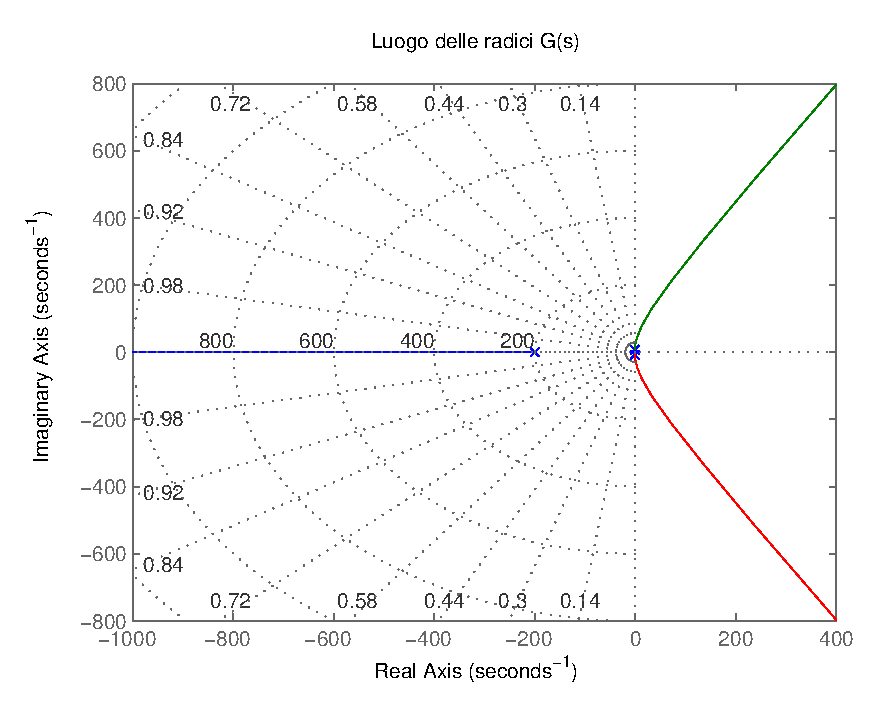
\includegraphics [width=4in]{prog6RADICI_02.eps}


\subsection*{Analisi del luogo delle radici di $ G(s) $ }

\begin{par}
Il luogo delle radici evidenzia le posizioni dei poli della funzione In particolare mostra che esiste un polo a parte reale negativa in $ -200 \frac{rad}{s} $ .
Ed inoltre mostra come vi siano due poli complessi e coniugati molto vicini allo zero, che cioè domineranno l'andamento del sistema.
\end{par} \vspace{1em}


\subsection*{Analisi sistema: scelta del regolatore}

\begin{par}
Il regolatore sarà formato da due parti (oltre a quella che annulla il sistema):
Una, $ RegS(s) $ , relativa al soddisfacimento delle specifiche statiche.
L'altra,  $ RegD(s) $, relativa al soddisfacimento della specifiche dinamiche.
\end{par}


\subsection*{1. Specifiche statiche}

\begin{par}
Errore a regime nullo in presenza di ingresso di riferimento a gradino di ampiezza massima pari a 2
e disturbo sull'uscita a gradino di ampiezza massima pari a 0.2.
\end{par}


\subsection*{1.1. Soluzione:}

\begin{par}
Dall'analisi della funzione di sensitività  $ S(s) = \frac{1}{1 + L}  $, è noto che
per avere errore a regime nullo, in risposta ad un ingresso a scalino di ampiezza A
è necessario che la funzione d'anello  abbia almeno un polo nell'origine.
Cioè vale la relazione:
$$ e_\infty = lim_{s \to 0} sS(s)\frac{A}{s} = A lim_{s \to 0} \frac{s^g}{s^g + \mu} = 0 \\, g > 0 $$
Questo risultato è valido in virtù del fatto che  S(s)  rappresenta la
funzione di trasferimento tra il riferimento e l'errore.
Inoltre, dato che la funzione di sensitività, rappresenta anche la
funzione di trasferimento, cambiata di segno, tra l'errore ed il
disturbo, ed in questo caso cerchiamo errore a regime nullo, allora
imporre la condizione in cui $ RegS(s) = \frac{\mu_s}{s} $ risolve entambi i problemi.


$ \mu_s  $ può essere un qualsiasi parametro libero, in quanto $ RegS(s) $  ha un polo
nell'origine indipendentemente dal valore dell'ampiezza dell'ingresso di
riferimento
\end{par}

\begin{verbatim}

us = 1; % 1 a default
RegS = us/s;
disp('RegS');
RegS

% Allora definisco il sistema esteso G_e(s) = G(s) RegS(s)
Ge = G * RegS;

% Che sarà la funzione che verrà considerata per il progetto del regolatore dinamico
\end{verbatim}

        \color{lightgray} \begin{verbatim}RegS

RegS =
 
  1
  -
  s
 
Continuous-time transfer function.

\end{verbatim} \color{black}
    

\subsection*{2. Specifiche dinamiche}

\begin{par}
\begin{itemize}
\setlength{\itemsep}{-1ex}
   \item 2) Massima sovraelongazione della risposta al riferimento a gradino inferiore al 5%.
   \item 3) Tempo di assestamento al 1% della risposta al gradino di riferimento, inferiore a 1.0 s
   \item 4) Margine di fase superiore a 45 gradi, per garantire robustezza.
\end{itemize}
\end{par}


\subsection*{2.1. Soluzione:}

\begin{par}
Dall'analisi delle posizione delle singolarità di G, notiamo che esiste un polo a
parte reale negativa in $ -200 \frac{rad}{s} $ e vi siano due poli complessi e coniugati molto vicini allo zero, che domineranno
l'andamento del sistema.

Per questo motivo, è possibile approssimare la risposta allo scalino,
con quella di un sistema $ Ga(s) $ , la cui funzione di trasferimento è
possiede soltanto questi poli dominante ed un guadagno statico pari a quello
del sistema di partenza.

Ricordando che l'approssimazione a poli dominanti è valida solo se le due
funzioni hanno pari guadagno statico

Definisco $ Ga(s) $, facendo in modo che il guadagno statico sia lo
stesso di $ G(s) $
\end{par}
\begin{verbatim}
Ga = (60 * u_stat) /(s^(2) + 2*s + 60);
disp('Guadagno statico di Ga: ');
disp(dcgain(Ga));
\end{verbatim}

\begin{par}

Quindi il sistema in esame (per quanto riguarda la risposta allo scalino) diventa un sistema con poli complessi coniugati, del quale sono note formule che possono semplificare il progetto.

\end{par}
\begin{verbatim}

figure(4); % Creo un altro oggetto grafico

% Mostro la risposta allo scalino di ampiezza 2 del sistema originario e
% del sistema approssimante.
% In giallo rosso l'originario, in nero tratteggiato l'approssimazione

step(2*G, 'r:', 2*Ga, 'b--');

grid on; % Attivo la visualizzazione della griglia
title('Risposta al gradino di ampiezza 2 -> G(s) (red) e Ga(s) (black dashed)');
\end{verbatim}

\begin{par}

Quindi utilizzando il sistema $ Ga(s) $, approssimante di $ G(s) $, è noto che per un sistema
con poli complessi coniugati la sovraelogazione percentuale è data da:
$$ S_{\%} = 100e^{\frac{-\pi \xi}{\sqrt{1 - \xi^2}}} $$
dove $ \xi $ indica lo smorzamento dei poli.
Quindi, per soddisfare il requisito, è necessario che: $ S_{\%} <= 5 $
Per cui è necessario che $ \xi >= 0.69 \approx 0.7 $
Dato che lo smorzamento è legato al margine di fase dalla relazione:
$ \xi = \frac{Mf \pi}{2 \times 180} \approx \frac{Mf}{100} $ la specifica sulla sovraelongazione richiede quindi un
margine di fase minimo.
In particolare vogliamo che il margine di fase sia $ \approx 100 \xi >= 70 grad $
Quindi, soddisfacendo questo vincolo, riusciamo anche a soddisfare il punto 4
\end{par}

\begin{verbatim}
xi = 0.7;
Mf_min = 70;
\end{verbatim}

\begin{par}
Il tempo di assistamento richiesto offre indicazioni sulla pulsazione critica:
$$ \xi \omega_n >= \frac{4.6}{T_{as}} => \omega_n >= \frac{4.6}{\xi \times 1} = 6,57 $$
Cioè la specifica ci chiede che il diagramma delle ampiezze di della
funzione d'anello intersechi l'asse a 0db, a pulsazioni superiori a $ 6,6 \frac{rad}{s} $ .
Ma dall'analisi del grafico di $ G(s) $  sappiamo che è consigliabile
scegliere una pulsazione critica per valori superiori o uguali a 11,
quindi
\end{par}
\begin{verbatim}
wc = 11;
\end{verbatim}

        \color{lightgray} \begin{verbatim}Guadagno statico di Ga: 
    1.5000

\end{verbatim} \color{black}
    
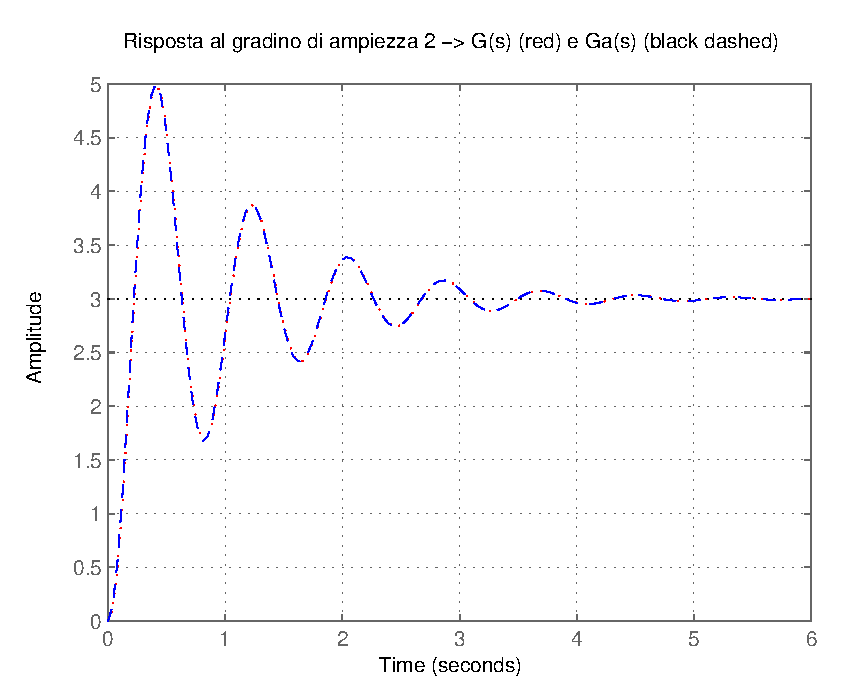
\includegraphics [width=4in]{prog6RADICI_03.eps}


\subsection*{2.1.2. Analisi di $ G_e(s) $ }

\begin{verbatim}
figure(4);
[GeGm, GePm] = margin(Ge);
disp('Margine di guadagno: '); disp(GeGm);
disp('Margine di fase: '); disp(GePm);
margin(Ge);
grid on;
\end{verbatim}
\begin{par}

Dall'analisi si evince che nelle vicinanze di $ \omega_c $ abbiamo una fase pessima (circa -250).

Per migliorare il margine di fase, è naturale pensare ad una rete anticipatrice.

In questo caso, dato che dal grafico di $ Ge(s) $ è noto che $ Arg(Ge(j\omega_{c}^*) = -256 $ 
la rete anticipatrice dovrà avere un anticipo di almeno $ 256 - ( 180 - 70) =  146 grad $, che con una singola rete anticipatrice non è possible.
\end{par}

        \color{lightgray} \begin{verbatim}Margine di guadagno: 
    1.3221

Margine di fase: 
   86.4480

\end{verbatim} \color{black}
    
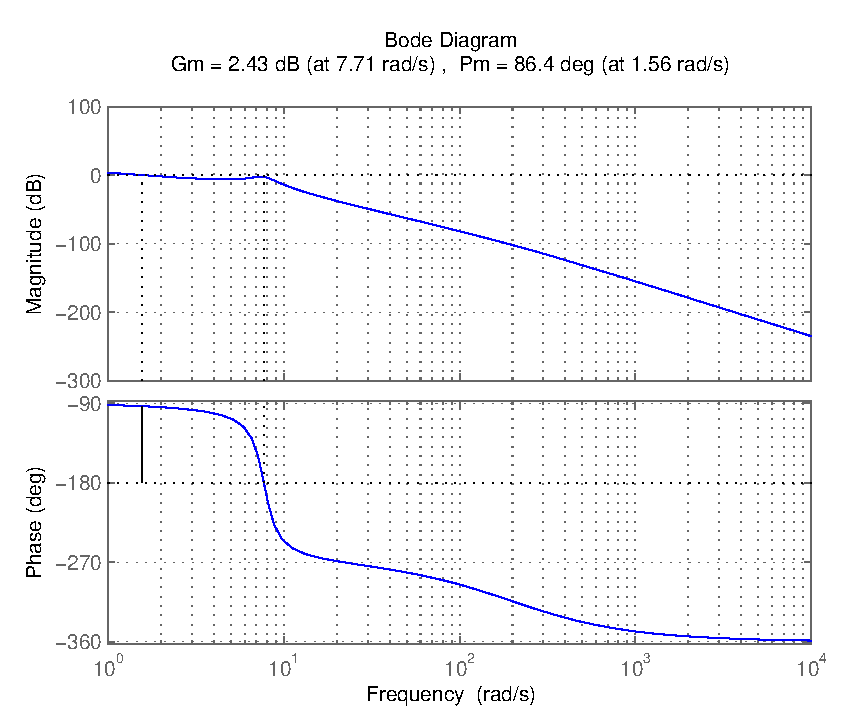
\includegraphics [width=4in]{prog6RADICI_04.eps}


\subsection*{Progetto}



\subsection*{3.1 Progetto Rete Anticipatrice Doppia}

\begin{par}
Allora si potrebbe progettare una rete anticipatrice doppia, in modo da
ottenere questo anticipo.

Si richiederebbe che ogni rete anticipatrice debba anticipare di
almeno 73 gradi.

Inoltre è necessaria un'amplificazione del modulo di $ Ge(s) $ tale da
permettere l'attraversamento dello zero in $ \omega_c $
Quindi ogni rete amplificatrice dovrà amplificare di $  \approx 9_{db}  $

Anziché procedere per tentativi, utilizzo un algoritmo evoluto basato sui
diagrammi di sfasamento e amplificazione.

Uso le coppie di poli e zeri, rispettivamente coincidenti per comodità.
Quindi ricerco un regolatore nella forma:

$$ RegD(s) = \frac{(1 + \tau s)^2}{(1 + \alpha \tau s)^2}, \\ 0 < \alpha < 1 $$
\end{par}


\subsection*{3.1.2 Diagrammi di sfasamento e amplificazione}

\begin{verbatim}
% plottiamo i diagrammi di amplificazione e sfasamento utili

de=logspace(-2,0); % definisco asse x con le pulsazioni normalizzate

% livello di amplificazione:

% alpha per cui tracciare il grafico
alpha_a=[0.001 0.005 0.008 0.01 0.05 0.15 0.25 0.35 0.45 0.55 0.65 0.75 0.85];

figure(7)

for i = 1:length(alpha_a)
    mod_R=10*log10((1+de.^2/alpha_a(i))./(1+de.^2*alpha_a(i)));
    loglog(de,mod_R);
    hold on;
end

grid on
title('Livello Amplificazionè)
xlabel('deltà)
ylabel('dB')

% entità sfasamento positivo:

alpha_int=0.05;

for i = 2:18
    alpha_int(i)=alpha_int(i-1)+0.05;
end

alpha_s=[0.001 0.005 0.008 0.01 alpha_int]; % alpha per cui tracciare il grafico

figure(8)

for i = 1:length(alpha_s)
    gr_R_rad=atan(de./sqrt(alpha_s(i)))-atan(de.*sqrt(alpha_s(i)));
    gr_R_gradi=gr_R_rad.*(180/pi);
    semilogx(de,gr_R_gradi);
    hold on;
end

grid on
title('Entità Sfasamentò)
xlabel('deltà)
ylabel('gradì)
\end{verbatim}

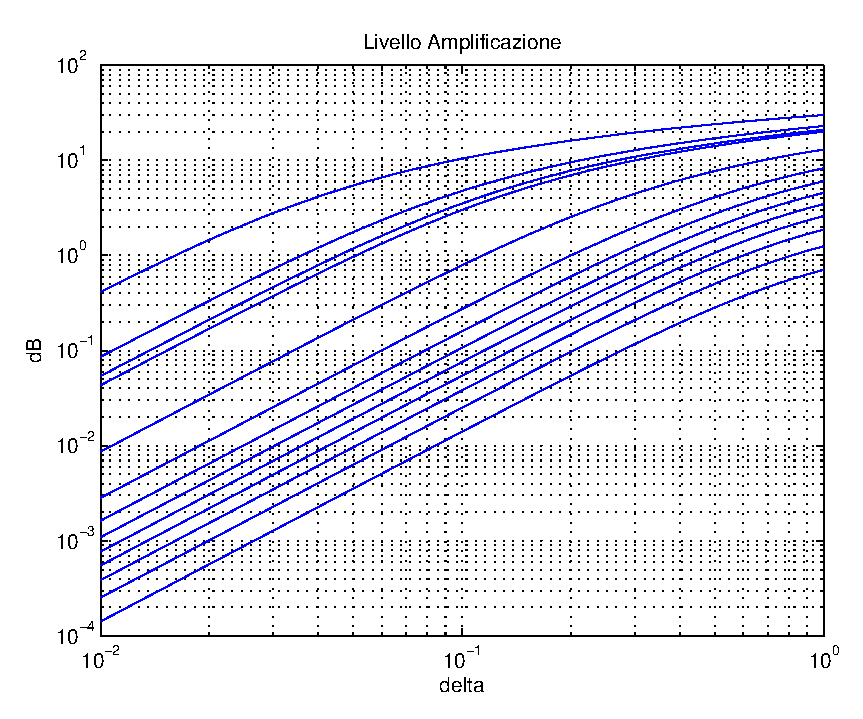
\includegraphics [width=4in]{prog6RADICI_05.eps}

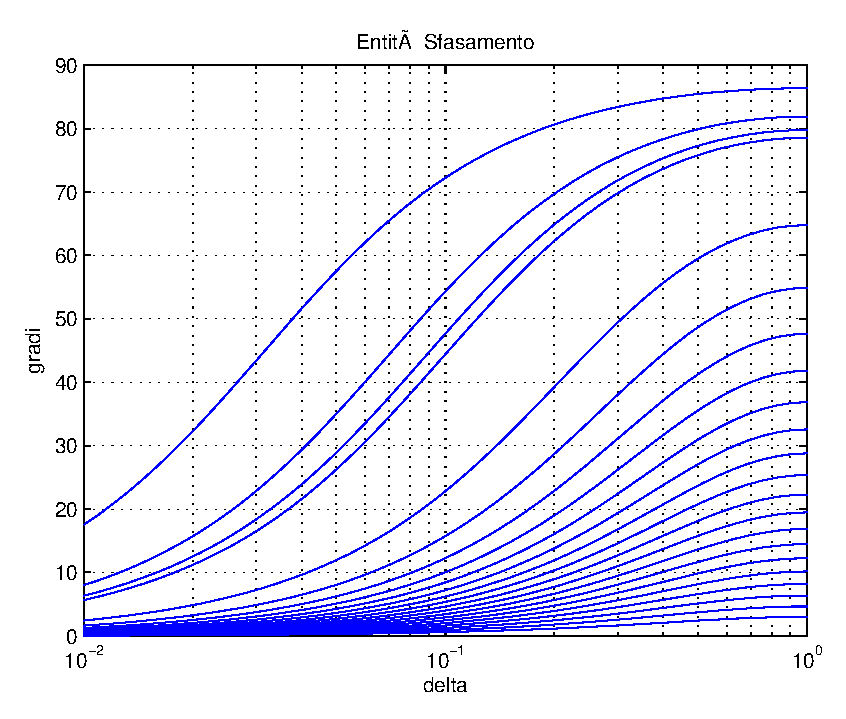
\includegraphics [width=4in]{prog6RADICI_06.eps}


\subsection*{3.1.3. Ricerca della coppia soddisfacente le specifiche.}

\begin{par}
Dall'analisi del grafico risulta che non esiste una coppia $ (\alpha^*, \delta^*) $che soddisfi le condizioni.
\end{par}


\subsection*{3.2. Rete anticipatrice tripla}

\begin{par}
Decido quindi di creare una rete d'anticipo tripla, in cui sono stati scelti poli
e zeri complessi coniugati coincidenti, per comodità.

Supponiamo che ogni rete debba recuperare 50 gradi e 6 db.
Allora uso i diagrammi di amplificazione e sfasamento per trovare la coppia
$ (\alpha^{*}, \delta^{*}) $ soddisfacente le condizioni.
Quindi ricerco un regolatore nella forma:

$$ RegD(s) = \frac{(1 + \tau s)^3}{(1 + \alpha \tau s)^3}, \\ 0 < \alpha < 1 $$
\end{par}


\subsection*{3.2.1 Ricerca della coppia soddisfacente}

\begin{par}
Dall'analisi del grafico del livello di amplificazione, noto che i punti
che intersecano l'asse a 6db, sono:

$$ \alpha : [0.001 0.005 0.01 0.05 0.15] $$
$$ \alpha = 0.001 \rightarrow \delta = 0.055 $$
$$ \alpha = 0.005 \rightarrow  \delta = 0.12 $$
$$ \alpha = 0.01  \rightarrow  \delta = 0.17 $$
$$ \alpha = 0.05  \rightarrow  \delta = 0.39 $$
$$ \alpha = 0.15  \rightarrow  \delta = 0.69 $$
$$ \alpha = 0.25  \rightarrow  \delta = 1 $$

Ora controllo nel grafico dell'entità di sfasamento se esiste una coppia
$ (\alpha^{*}, \delta^{*}) $  che fornire lo sfasamento da noi desiderato $ \approx 50 $

Quindi,

Per $ \delta = 0.087 $  si ha uno sfasamento di circa 50 grad
Per $ \delta = 0.12 $ si ha uno sfasamento di circa 50 grad

Qui mi fermo, dato che ho trovato una coppia che soddisfa amplificazione e sfasamento necessario.
\end{par}
\begin{verbatim}

alpha = 0.005;
delta = 0.12;

% Allora, si ha

tau = delta / (wc * sqrt(alpha));

us = 1; % il guadagno è ancora libero

RegD = us*( ( ((1+tau*s)^3) ) / (( (1+ alpha*tau*s)^3) ));

R = RegS * RegD;

L = R * G;
\end{verbatim}


\subsection*{3.2.2. Verifica risultati}

\begin{par}
Controllo i margini della nuova funzione di retroazione
\end{par}

\begin{verbatim}

figure(3);
margin(L);
[GeGm, GePm, Wgm, Wpm] = margin(L);

if GePm > Mf_min
    disp ('[OK] Margine di fase valido: ');
else
    disp ('[!] Specifica relativa allo smorazamento NON rispettata: ');
end
disp(GePm);

if Wpm > wc
    disp('[OK] Frequenza a guadagno unitario: ');
    disp(Wpm);
else
    disp ('[!] Vincolo sulla pulsazione critica non rispettato: ');
end

disp (Wpm);

% Con questi valori, si ha un anomalo doppio attraversamento dello zero,
% quindi calcolo un guadagno appropriato, dopo alcuni tentativi ottengo:

us = 10^(7.7/20);

% Quindi il regolatore dinamico diventa

RegD = us*( ( ((1+tau*s)^3) ) / (( (1+ alpha*tau*s)^3) ));

R = RegS * RegD;

L = R * G;

% Controllo nuovamente
figure(31);
margin(L);
[GeGm, GePm, Wgm, Wpm] = margin(L);

if GePm > Mf_min
    disp ('[OK] Margine di fase valido: ');
else
    disp ('[!] Specifica relativa allo smorazamento NON rispettata: ');
end
disp(GePm);

if Wpm > wc
    disp('[OK] Frequenza a guadagno unitario: ');
    disp(Wpm);
else
    disp ('[!] Vincolo sulla pulsazione critica non rispettato: ');
end

disp (Wpm);
\end{verbatim}

\begin{verbatim}

% Mostro la risposta al gradino del sistama retroazionato

figure(9);
title('Risposta al gradino di riferimento del sistema retroazionatò);

% Quindi il sistema è dato dalla funzione feedback, dove il prima termine
% rapresenta la funzione di trasferimento del sistema in catena diretta, il
% secondo quello in retroazione

step(2 * feedback(L,1));

disp('L'); L
\end{verbatim}

        \color{lightgray} \begin{verbatim}[OK] Margine di fase valido: 
  103.4742

[!] Vincolo sulla pulsazione critica non rispettato: 
   10.8310

[OK] Margine di fase valido: 
  128.9249

[OK] Frequenza a guadagno unitario: 
   23.1217

   23.1217

L

L =
 
                                                            
                160.4 s^3 + 3119 s^2 + 2.022e04 s + 4.368e04
                                                            
  ------------------------------------------------------------------------
                                                                          
  4.59e-10 s^7 + 1.878e-06 s^6 + 0.002675 s^5 + 1.468 s^4 + 203.1 s^3     
                                                                          
                                                     + 487.8 s^2 + 12000 s
                                                                          
 
Continuous-time transfer function.

\end{verbatim} \color{black}
    
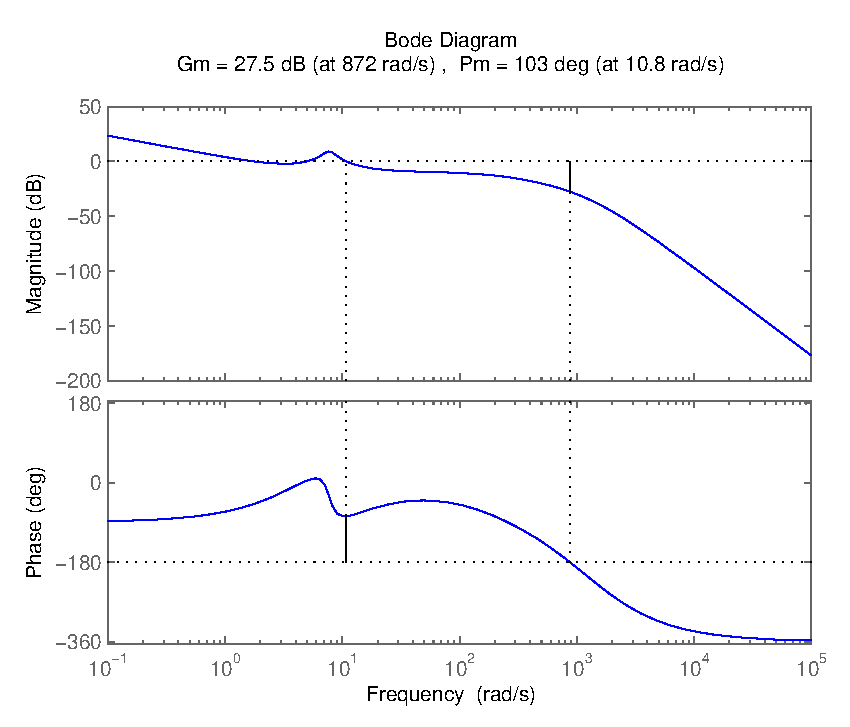
\includegraphics [width=4in]{prog6RADICI_07.eps}

\includegraphics [width=4in]{prog6RADICI_08.eps}

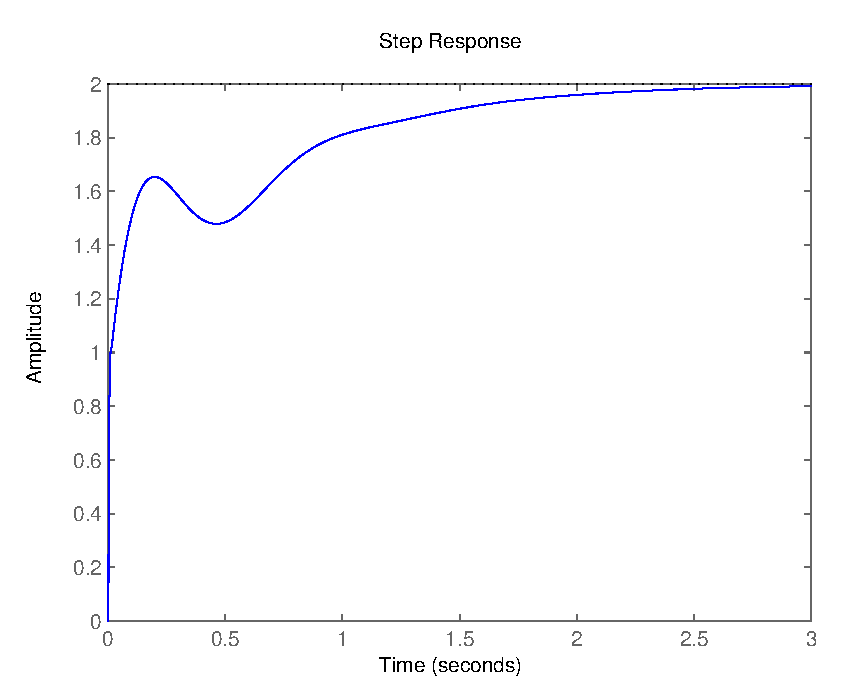
\includegraphics [width=4in]{prog6RADICI_09.eps}

\begin{par}
Avendo scelto questo guadagno, si ha $ \omega_c \approx 23.1 \frac{rad}{s} $ ed il margine di fase corretto.

Tutte le specifiche frequenziali sono state rispettate.
L'unica cosa che non si rispetta è il tempo di assestamento ( che è attorno ai 4 secondi).
\end{par}

\subsection*{3.2.3. Analisi del luogo delle radici}

\begin{par}
Analizziamo il luogo delle radici della funzione d'anello.
\end{par}
\begin{verbatim}

figure(11);
rlocus(L);
axis([-50 3 -15 15]);
\end{verbatim}
\begin{par}
Per ridurre il tempo di assestamento provo a ricalibrare la rete di
ritardo creata, in modo da allontanare ulteriormente gli zeri dall'origine.
I quali, probabilmente, vengono attratti dal polo posto nel regolatore
statico e fanno sì che si crei l'esponenziale lento che genera la coda di
assestamento.
\end{par}

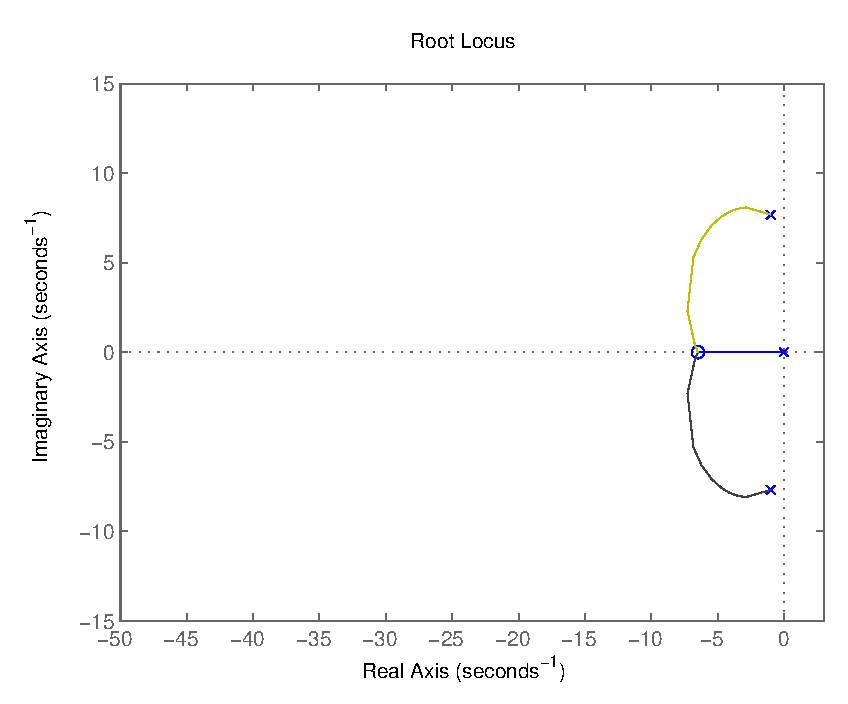
\includegraphics [width=4in]{prog6RADICI_10.eps}


\subsection*{3.2.4. Ricalibrazione}

\begin{par}
Dato che il guadango del sistema è libero, è facile imporre una pulsazione
di attraversamento variando opportunamente il valore del guadagno.

Visto che non ho vincoli (al momento), relativi al limite superiore della pulsazione critica e
che questa figura all'interno del calcolo dei coefficienti della rete di
anticipo, scelgo di imporre una pulsazione di attraversamento maggiore, $ \omega_c  = 21 $ , successivamente, agendo sul guadango, potrò fissare la pulsazione di taglio desiderata.
\end{par}
\begin{verbatim}
wc = 21;

tau = delta / (wc * sqrt(alpha));

% Dopo alcuni tentativi, trovo che il guadagno ideale è

us = 10^(22.6/20);

RegD = us*( ( ((1+tau*s)^3) ) / (( (1+ alpha*tau*s)^3)));

R = RegS * RegD;

L = R * G;

figure(99);

margin(L);

% mostro la risposta al gradino

figure(888);
step(2 * feedback(L,1));
\end{verbatim}
\begin{par}
La risposta è buona, ora rispetta il tempo di assestamento.
Il vincolo sulla sovraelongazione non è più rispettato, ma ovvierò a questo inconveniente mediante una rete di compensazione (vedi dopo).
\end{par}

\includegraphics [width=4in]{prog6RADICI_11.eps}

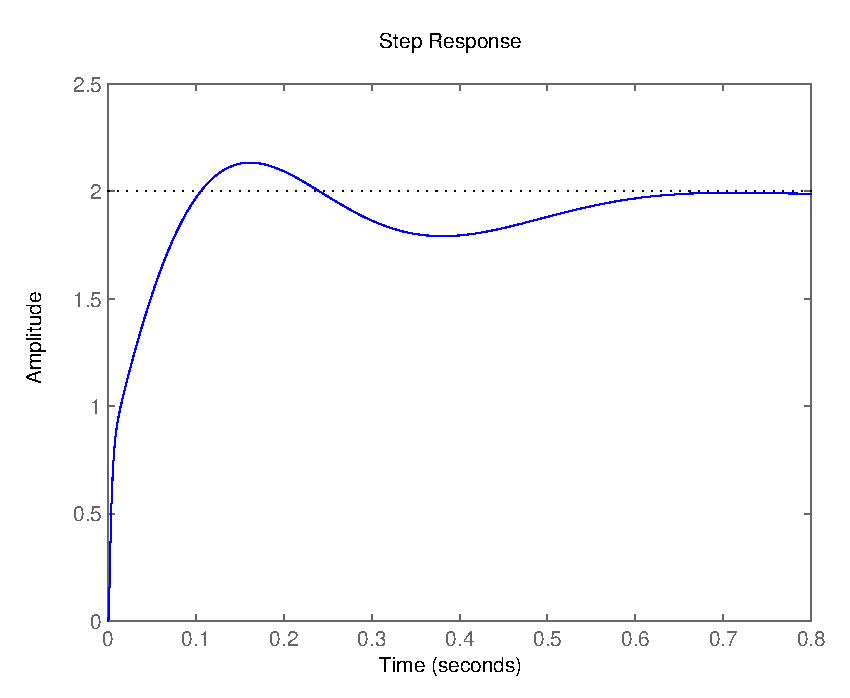
\includegraphics [width=4in]{prog6RADICI_12.eps}


\subsection*{Rumore di misura ad alta frquenza}

\begin{par}
Per tenere in conto del rumore di misura ad alte frequenze, introduco
nel regolatore dinamico 3 poli ad alta frequenza che eliminano
dall'uscita l'influenza del rumore.
Li posiziono tatticamente una decade prima del rumore di misura.
\end{par}
\begin{verbatim}

RegD = RegD / (((1 + 0.004*s)^3));

R = RegS * RegD; % Ridefinisco il regolatore

L = R * G; % Ridefinisco R

[LGm, LPm, Wgm, Wpm] = margin(L);
figure(666);
margin(L);

figure(999);
step(2 * feedback(L,1));
\end{verbatim}
\begin{par}
L'introduzione dei poli non ha modificato moltissimo le specifiche frequenziali, che risultano tutt'ora rispettate.

\end{par}

\includegraphics [width=4in]{prog6RADICI_13.eps}

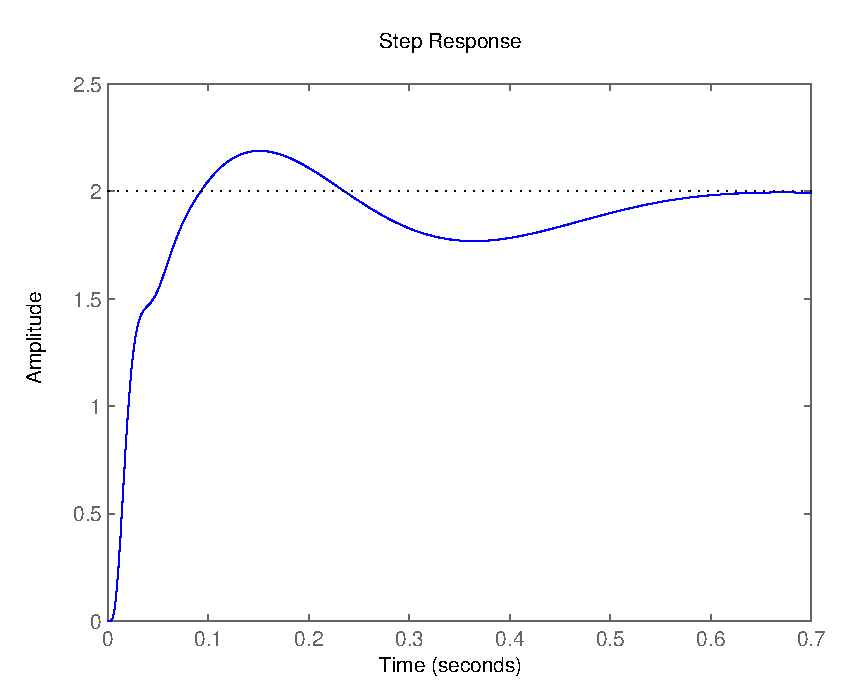
\includegraphics [width=4in]{prog6RADICI_14.eps}


\subsection*{4. Simulink}

\begin{par}
Inserisco un pre-filtro, in modo da eseguire un'operazione di pre-fitraggio del segnale di riferimento, cioè
in modo da alterare le compoenenti frequenziali di questo che sono iniettate nel sistema in retroazione.

Ricordando che
$$ Y(s) = \frac{R(s)G(s)}{1 + R(s)G(s)}C(s)W(s) = F(s)C(s)W(s) $$
e che
$$ U(s) = \frac{R(s)}{1 + R(s)G(s)}C(s)W(s) = Q(s)C(s)W(s) $$
Allora con il compensatore C (definito PF in Matlab) posso modificare:
1. La funzione di trasferimento fra il riferimento e l'uscita
2. La funzione di trasferimento tra il riferimento e la variabile di controllo

Scegliendo un compensatore nella forma:
$$ C(s) = \frac{\omega_a}{\omega_a  + s} $$
Dove $ \omega_a $ è scelta in modo da far agire il polo del
compensatore lievemente in anticipo rispetto alla pulsazione critica del
regolatore, in modo da attenuare le componenti spettrali in ingresso, riducendo la sovraelongazione.
Questo a discapito del tempo di assestamento, nel quale, però, eravamo già ampliamente in specifica.

Scegliendo $ \omega_a = \frac{\omega_c}{1.1} $
riesco a rispettare tutte le specifiche di progetto.
\end{par}
\begin{verbatim}
wc = Wpm;
wa = wc / 1.1;

PF = wa / ( wa + s);
\end{verbatim}


\subsection*{4. Funzioni di sensititività}

\begin{verbatim}
% Funzione di sensitività complementare
F = minreal(L/(1+L));
figure(5);
bode(F, P);
grid on;
title('Funzione di sensitività' complementarè);

% Funzione di sensitività
S = minreal(1/(1+L));
figure(5);
bode(S, P);
grid on;
title('Funzione di sensitività'');

% Funzione di sensitività del controllo
Q = minreal(R/(1+L));
figure(6);
bode(Q, P);
grid on;
title('Funzione di sensitività' del controllò);
\end{verbatim}

\includegraphics [width=4in]{prog6RADICI_15.eps}

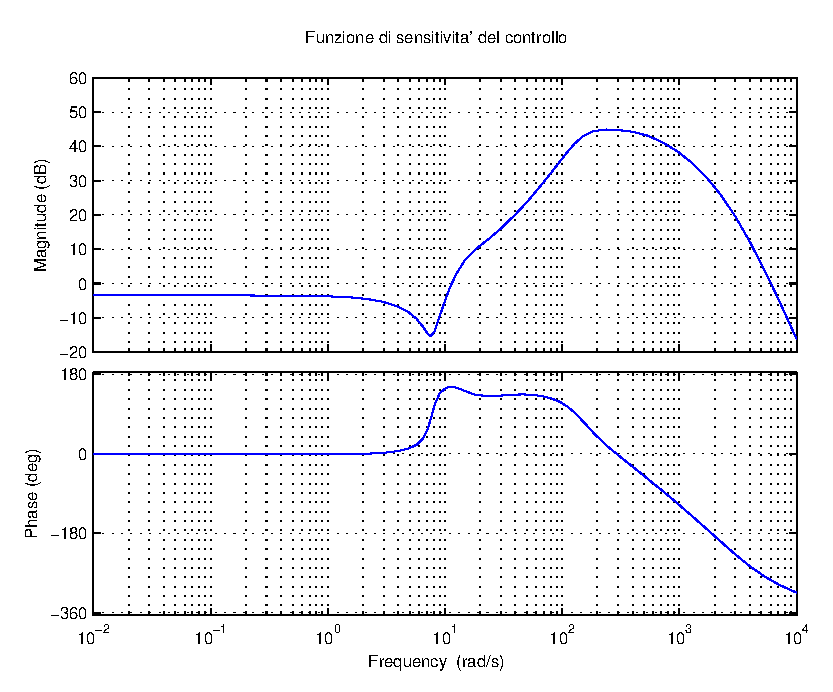
\includegraphics [width=4in]{prog6RADICI_16.eps}


\subsection*{4.1 Schema di simulazione}

\begin{par}
\includegraphics[width=\paperwidth,height=\textheight,keepaspectratio, angle=90]{prog6RADICI_17.eps}
\end{par} \vspace{1em}


\subsection*{4.1 Simulazione}

\begin{par}
\includegraphics[width=\paperwidth,height=\textheight,keepaspectratio, angle=90]{simulazione.eps}
\includegraphics[width=\paperwidth,height=\textheight,keepaspectratio, angle=90]{sovraelonga.eps}
\end{par} \vspace{1em}
\begin{par}
Osservando attentamente la simulazione si nota come tutti i parametri e le specifiche di
progetto vengano rispettate correttamente. Come intervallo della saturazione dell'attuatore
vengono scelti i valori [-4.5, 14.5] al fine di garantire la corretta gestione del transitorio.
\end{par}


\end{document}
    
